\documentclass{beamer}

% xcolor and define colors -------------------------
\usepackage{xcolor}

% https://www.viget.com/articles/color-contrast/
\definecolor{purple}{HTML}{5601A4}
\definecolor{navy}{HTML}{0D3D56}
\definecolor{ruby}{HTML}{9a2515}
\definecolor{alice}{HTML}{107895}
\definecolor{daisy}{HTML}{EBC944}
\definecolor{coral}{HTML}{F26D21}
\definecolor{kelly}{HTML}{829356}
\definecolor{cranberry}{HTML}{E64173}
\definecolor{jet}{HTML}{131516}
\definecolor{asher}{HTML}{555F61}
\definecolor{slate}{HTML}{314F4F}

% Mixtape Sessions
\definecolor{picton-blue}{HTML}{00b7ff}
\definecolor{violet-red}{HTML}{ff3881}
\definecolor{sun}{HTML}{ffaf18}
\definecolor{electric-violet}{HTML}{871EFF}

% Main theme colors
\definecolor{accent}{HTML}{00b7ff}
\definecolor{accent2}{HTML}{871EFF}
\definecolor{gray100}{HTML}{f3f4f6}
\definecolor{gray800}{HTML}{1F292D}


% Beamer Options -------------------------------------

% Background
\setbeamercolor{background canvas}{bg = white}

% Change text margins
\setbeamersize{text margin left = 15pt, text margin right = 15pt} 

% \alert
\setbeamercolor{alerted text}{fg = accent2}

% Frame title
\setbeamercolor{frametitle}{bg = white, fg = jet}
\setbeamercolor{framesubtitle}{bg = white, fg = accent}
\setbeamerfont{framesubtitle}{size = \small, shape = \itshape}

% Block
\setbeamercolor{block title}{fg = white, bg = accent2}
\setbeamercolor{block body}{fg = gray800, bg = gray100}

% Title page
\setbeamercolor{title}{fg = gray800}
\setbeamercolor{subtitle}{fg = accent}

%% Custom \maketitle and \titlepage
\setbeamertemplate{title page}
{
    %\begin{centering}
        \vspace{20mm}
        {\Large \usebeamerfont{title}\usebeamercolor[fg]{title}\inserttitle}\\
        {\large \itshape \usebeamerfont{subtitle}\usebeamercolor[fg]{subtitle}\insertsubtitle}\\ \vspace{10mm}
        {\insertauthor}\\
        {\color{asher}\small{\insertdate}}\\
    %\end{centering}
}

% Table of Contents
\setbeamercolor{section in toc}{fg = accent!70!jet}
\setbeamercolor{subsection in toc}{fg = jet}

% Button 
\setbeamercolor{button}{bg = accent}

% Remove navigation symbols
\setbeamertemplate{navigation symbols}{}

% Table and Figure captions
\setbeamercolor{caption}{fg=jet!70!white}
\setbeamercolor{caption name}{fg=jet}
\setbeamerfont{caption name}{shape = \itshape}

% Bullet points

%% Fix left-margins
\settowidth{\leftmargini}{\usebeamertemplate{itemize item}}
\addtolength{\leftmargini}{\labelsep}

%% enumerate item color
\setbeamercolor{enumerate item}{fg = accent}
\setbeamerfont{enumerate item}{size = \small}
\setbeamertemplate{enumerate item}{\insertenumlabel.}

%% itemize
\setbeamercolor{itemize item}{fg = accent!70!white}
\setbeamerfont{itemize item}{size = \small}
\setbeamertemplate{itemize item}[circle]

%% right arrow for subitems
\setbeamercolor{itemize subitem}{fg = accent!60!white}
\setbeamerfont{itemize subitem}{size = \small}
\setbeamertemplate{itemize subitem}{$\rightarrow$}

\setbeamertemplate{itemize subsubitem}[square]
\setbeamercolor{itemize subsubitem}{fg = jet}
\setbeamerfont{itemize subsubitem}{size = \small}







% Links ----------------------------------------------

\usepackage{hyperref}
\hypersetup{
  colorlinks = true,
  linkcolor = accent2,
  filecolor = accent2,
  urlcolor = accent2,
  citecolor = accent2,
}


% Line spacing --------------------------------------
\usepackage{setspace}
\setstretch{1.2}


% \begin{columns} -----------------------------------
\usepackage{multicol}


% Fonts ---------------------------------------------
% Beamer Option to use custom fonts
\usefonttheme{professionalfonts}

% \usepackage[utopia, smallerops, varg]{newtxmath}
% \usepackage{utopia}
\usepackage[sfdefault,light]{roboto}

% Small adjustments to text kerning
\usepackage{microtype}



% Remove annoying over-full box warnings -----------
\vfuzz2pt 
\hfuzz2pt


% Table of Contents with Sections
\setbeamerfont{myTOC}{series=\bfseries, size=\Large}
\AtBeginSection[]{
        \frame{
            \frametitle{Roadmap}
            \tableofcontents[current]   
        }
    }


% Tables -------------------------------------------
% Tables too big
% \begin{adjustbox}{width = 1.2\textwidth, center}
\usepackage{adjustbox}
\usepackage{array}
\usepackage{threeparttable, booktabs, adjustbox}
    
% Fix \input with tables
% \input fails when \\ is at end of external .tex file
\makeatletter
\let\input\@@input
\makeatother

% Tables too narrow
% \begin{tabularx}{\linewidth}{cols}
% col-types: X - center, L - left, R -right
% Relative scale: >{\hsize=.8\hsize}X/L/R
\usepackage{tabularx}
\newcolumntype{L}{>{\raggedright\arraybackslash}X}
\newcolumntype{R}{>{\raggedleft\arraybackslash}X}
\newcolumntype{C}{>{\centering\arraybackslash}X}

% Figures

% \imageframe{img_name} -----------------------------
% from https://github.com/mattjetwell/cousteau
\newcommand{\imageframe}[1]{%
    \begin{frame}[plain]
        \begin{tikzpicture}[remember picture, overlay]
            \node[at = (current page.center), xshift = 0cm] (cover) {%
                \includegraphics[keepaspectratio, width=\paperwidth, height=\paperheight]{#1}
            };
        \end{tikzpicture}
    \end{frame}%
}

% subfigures
\usepackage{subfigure}


% Highlight slide -----------------------------------
% \begin{transitionframe} Text \end{transitionframe}
% from paulgp's beamer tips
\newenvironment{transitionframe}{
    \setbeamercolor{background canvas}{bg=accent!40!black}
    \begin{frame}\color{accent!10!white}\LARGE\centering
}{
    \end{frame}
}


% Table Highlighting --------------------------------
% Create top-left and bottom-right markets in tabular cells with a unique matching id and these commands will outline those cells
\usepackage[beamer,customcolors]{hf-tikz}
\usetikzlibrary{calc}
\usetikzlibrary{fit,shapes.misc}

% To set the hypothesis highlighting boxes red.
\newcommand\marktopleft[1]{%
    \tikz[overlay,remember picture] 
        \node (marker-#1-a) at (0,1.5ex) {};%
}
\newcommand\markbottomright[1]{%
    \tikz[overlay,remember picture] 
        \node (marker-#1-b) at (0,0) {};%
    \tikz[accent!80!jet, ultra thick, overlay, remember picture, inner sep=4pt]
        \node[draw, rectangle, fit=(marker-#1-a.center) (marker-#1-b.center)] {};%
}

\usepackage{breqn} % Breaks lines

\usepackage{amsmath}
\usepackage{mathtools}
\usepackage{subcaption}

\usepackage{pdfpages} % \includepdf

\usepackage{listings} % R code
\usepackage{verbatim} % verbatim

% Video stuff
\usepackage{media9}

% packages for bibs and cites
\usepackage{natbib}
\usepackage{har2nat}
\newcommand{\possessivecite}[1]{\citeauthor{#1}'s \citeyearpar{#1}}
\usepackage{breakcites}
\usepackage{alltt}

% tikz
\usepackage{tikz}
\usepackage{pgfplots}
\usetikzlibrary{calc, positioning, decorations.pathreplacing, arrows.meta, intersections}
\pgfdeclarelayer{bg}
\pgfdeclarelayer{back}
\pgfdeclarelayer{fg}
\pgfsetlayers{bg,main,fg,back}
\usetikzlibrary{shapes,arrows}

% Setup math operators
\DeclareMathOperator{\E}{E} \DeclareMathOperator{\tr}{tr} \DeclareMathOperator{\se}{se} \DeclareMathOperator{\I}{I} \DeclareMathOperator{\sign}{sign} \DeclareMathOperator{\supp}{supp} \DeclareMathOperator{\plim}{plim}
\DeclareMathOperator*{\dlim}{\mathnormal{d}\mkern2mu-lim}
\newcommand\independent{\protect\mathpalette{\protect\independenT}{\perp}}
   \def\independenT#1#2{\mathrel{\rlap{$#1#2$}\mkern2mu{#1#2}}}
\newcommand*\colvec[1]{\begin{pmatrix}#1\end{pmatrix}}

\newcommand{\myurlshort}[2]{\href{#1}{\textcolor{gray}{\textsf{#2}}}}


\begin{document}

\title{About Causal Inference and How It Can Improve Impact Evaluation of Takaful and Karama}
\author{by Scott Cunningham (Baylor University)}
\date{\today}

\begin{frame}
\titlepage
\end{frame}


\section{What is causal inference?}



\subsection{Core questions in causal inference}


%\begin{frame}{Introduction: About Me}
%\begin{itemize}
%\item I'm Scott Cunningham, the Ben H. Williams Professor of Economics at Baylor University
%\item Baylor is located in Waco, Texas: a small city in one of the USA's largest states by area and population.
%\item I'm the author of \underline{Causal Inference: the Mixtape}, as well as numerous articles in applied economics focusing on gender, crime, maternal health, drug policy, and mental illness and self harm in prisons and jails
%\item I'm honored and appreciative to be here with you all today.
%\end{itemize}
%\end{frame}

\begin{frame}{Overview of Today's Talk}
\begin{itemize}
\item Firstly, we'll explore \emph{causal inference}: 
    \begin{itemize}
    \item What is it?  Why is it important?  What is at stake? % what is the value added of the techniques in causal inference and what are examples of assessment. I need to use the 10 minutes to make the point for causal inference -- focusing on the range of methods. 
    \item Importance of \emph{controlled randomization} and options when we can't.
    \end{itemize}
\item Secondly, we'll delve into a 2018 evaluation by IFPRI:
    \begin{itemize}
    \item Focusing on the Takaful (Solidarity) and Karama (Dignity) programs.
    \item Understanding the evaluation's findings and implications.
    \end{itemize}
\end{itemize}
\end{frame}



%\begin{frame}{Important Distinctions: Correlation vs. Causal Inference}

%What is correlation?  When is it causal and when is it not? 

%\bigskip

%\begin{itemize}
%\item \emph{Correlation} is a purely statistical concept measuring movements between two things
%\item \emph{Causal Inference} uses in data, assumptions and statistical models to estimate causal effects
%\end{itemize}
%\end{frame}




%\begin{frame}{Metaphysics of Causality}
%\begin{itemize}
%\item Metaphysics is the study of what exists and the nature of that existence
%\item The metaphysics of causality seeks to define what it means for one event to cause another
%\item Explores the fundamental nature of the causal relationship
%\item Poses questions like: "What does it mean, fundamentally, for A to cause B?"
%\end{itemize}
%\end{frame}

%\begin{frame}{Epistemology of Causal Inference}
%\begin{itemize}
%\item Epistemology is the study of how we know what we know.
%\item The epistemology of causal inference focuses on how we infer causal relationships, or what it means for a causal belief to be credible
%\item Causal inference is focused on building useful methods that can be relied on to infer one thing caused another, as opposed to philosophical inquiries into the nature of reality
%\item We ask: "How can we reliably infer that our social programs caused the lives of poor people to improve?"
%\end{itemize}
%\end{frame}

\begin{frame}{Advances in causal inference}

\begin{itemize}
\item Causal inference is having its day in the sun
\item Explosion in advances in causal inference recently awarded with several major awards: 
	\begin{itemize}
	\item Josh Angrist, David Card and Guido Imbens (2021 Nobel Prize in Economics)
	\item Judea Pearl (2011 Turing Award in computer science)
	\item James Robins, Miguel Hernán, Thomas Richardson, Andrea Rotnitzky, and Eric Tchetgen Tchetgen (2022 Rousseeuw Prize for Statistics)
	\end{itemize}
\item Widespread adoption of causal inference for data driven decision making, both in government and commerce, has replaced simpler correlational methods
\item Exciting time!
\end{itemize}

\end{frame}



\begin{frame}{Examples of causal decisions}

Causal inference helps us know whether things work and by how much

 
\bigskip


\begin{itemize}
\item  Will mandatory vaccination laws reduce the spread of COVID?
\item  How will a new early reading curriculum impact youth literacy?  
\item  How much, if any, will cash transfers impact poor family's overall well-being?
\end{itemize}


\end{frame}


\begin{frame}{Counterfactuals and causal inference}

 Ladder of causation: observe relationships, intervene, and reason out the counterfactual

\bigskip

\textcolor{red}{Fundamental problem of causal inference}: We don't have anyone's counterfactuals because \emph{by definition} they never happened

\bigskip

Causal inference methods \emph{estimate} counterfactuals to understand intervention's impact but as counterfactuals don't exist, estimation require \emph{assumptions}, data and appropriate methods


\end{frame}



%\begin{frame}{Discerning causal effects}

%\begin{itemize}
%\item Gains from causal inference help us not only know whether things work (as opposed to driven by spurious and uninformative relationships found in our data sources) but also the magnitude
%\item Both are critical for designing policy when programs are very expensive and the goals are important
%\item Statistical methods are required but they are only as good as the assumptions beneath them -- no approach is “more scientific” if assumptions are not credible

%\end{itemize}

%\end{frame}



\begin{frame}{Correlations, Causal Effects, and Selection Bias}



\begin{itemize}
\item Imagine we find patients on ventilators have higher mortality than patients who aren't; two problems we face 
	\begin{enumerate}
	\item \textbf{Average causal effect}: Can we find the average effect of ventilators on mortality? If so how?
	\item \textbf{Selection bias}: How much of the observed differences between people on and off vents is because these the ventilator group always would've had higher mortality?
	\end{enumerate}
\item Our goal: find situations where we can credibly delete the second term so all that is left is the first term when comparing program participants to non-participants

\item Requires understanding the \emph{behavioral reason} people were selected, but some behavioral reasons for program participation make this a very difficult problem disentangle

\end{itemize}

\end{frame}


%  \begin{itemize}
%    \item Aliens from another planet come and notice that people on ventilators have higher mortality than those not on ventilators
%    \item They conclude that ventilators are killing people
%    \item Are they right?  Or  they have it backwards -- maybe doctors are putting sick people on ventilators to help them
%    \item How can separate the two?  By understanding the behaviors that drove people into and out of programs first and combining that with statistical methodologies that take advantage of that
%  \end{itemize}

%\end{frame}

%\begin{frame}{\#1: Correlation and causality are different concepts}

%  \begin{itemize}
%  	\item Differences between causality and correlation
%		\begin{itemize}
%	    \item Causal is about understanding the effect of one unit changing on another. ``If a person  puts a patient on a ventilator, will her covid symptoms improve?''
%	    \item Correlation, on the other hand, is about understanding relationships across many units. ``How do changes in ventilators relate to changes in covid symptoms across a population?''
%	    	\end{itemize}
%	\item Failure to understand the difference between causal inference and \emph{description} can lead to major errors in assessment and therefore policy recommendations
%  \end{itemize}  
%\end{frame}



%\begin{frame}{\#2: Coming first may not mean causality!}

%  \begin{itemize}
%    \item Every morning the rooster crows and then the sun rises
%    \item Did the rooster cause the sun to rise? Or did the sun cause the rooster to crow?
%    \item What if cat killed the rooster?  Would the sun never rise?
%    \item Simply assuming things happening one after another represents causal effects is an extension of the previous error
%  \end{itemize}

%\end{frame}

%\begin{frame}{\#3: Causality may mask correlations!}

%  \begin{figure}
%    \centering
%    \includegraphics[scale=0.04]{./lecture_includes/scottboat.jpg}
%  \end{figure}

%\end{frame}

\subsection{Treatment Assignment Mechanisms}


%\begin{frame}{Three New Ideas}

%\begin{enumerate}
%\item \textbf{Counterfactual}: Philosophers come to it first and its central role in causal inference makes causality \emph{unknowable} that the project is nearly derailed
%\item \textbf{Treatment assignment mechanism}: Neyman and Fisher solve the counterfactual problem in statistics and lay the foundation of the modern randomized controlled trial (RCT) %with their focus on the selection process
%\item \textbf{No One Causal Effect}: There is no such thing as ``the causal effect''; there's many and your first step is to pick a parameter (not as easy as it sounds)
%\end{enumerate}


%\end{frame}


% Rewrite this but without the equation.  Comparison = causal effect + selection bias

  




\begin{frame}{Spectrum of Treatment Assignment}

\begin{itemize}

%\item Treatment assignment \emph{mechanisms} refer to how and why a person participated into a program in the first place and the most common reason -- voluntary participation -- is a threat to causal inference
\item Ironically, the better run a program is, the more difficult it is to infer the effect 
% \item because humans naturally gravitate towards pleasure and away from pain (e.g., vents if COVID symptoms are severe)
\item Voluntary participation in well run programs become dominated by selection bias and may make it impossible to know average causal effects
\item Overcoming selection bias requires something external that put them into the program other than their own voluntary participation, but what?

\end{itemize}

\end{frame}




\begin{frame}{Randomization}
\begin{center}
\begin{tikzpicture}[node distance=2.5cm]
    % Nodes
    \node (Z) {Z (Lottery)};
    \node [below right of=Z] (T) {Vents};
    \node [right=3cm of T] (N) {Mortality};  % Adjusted distance here
    \node [right=1.5cm of Z] (U) {Severe illness};
    
    % Paths
    \draw[->] (Z) -- (T);
    \draw[->] (T) -- (N);
    \draw[->, dashed] (U) -- (T);
    \draw[->, dashed] (U) -- (N);
\end{tikzpicture}
\end{center}

\bigskip

\begin{itemize}
\item Randomized experiments are valuable for causal inference because program participation is \emph{not} based on voluntary participation, and therefore selection bias is minimized almost to nothing
\item But for some questions, the \emph{controlled} randomization may not be possible 
\item Randomized assignment of rural regions to good and bad schools would definitively measure the impact of schools on children, but this might be too expensive, infeasible or unethical to knowingly deprive some areas of crucial educational improvements
\end{itemize}



\end{frame}





\begin{frame}{Running Variables and Regression Discontinuity}
\begin{itemize}
\item But sometimes people were limited in their voluntary participation, not because they were in a controlled randomized experiment, but because their participation was based on a \emph{test} and their \emph{score}
\item When their \emph{grade} on a test is used to put them in a program, we call the test a \emph{running variable} and the eligibility a \emph{cutoff}
\item  Impact study by IFPRI published in 2018 used this method (also called \emph{regression discontinuity}) to study the impact of Takaful and Karama on a variety of health and life outcomes
\end{itemize}
\end{frame}

\begin{frame}{Methodology commentary}

\begin{itemize}
\item RDD is a design can under certain assumptions identify the average effect of the program on well being but \emph{only} for those people right above and below the eligibility cutoff
\item Insofar as those people differ from everyone else, the causal effects may lack external validity despite being true for those people
\item Method has a variety of techniques but at their core, they compare program participants who just barely got in because of some score they received on a running variable to those who just barely missed the cutoff
\item No more ``scientific'' or valid than any other method so long as the behavioral assignments meet the assumptions required for inference

\end{itemize}

\end{frame}


\section{Takaful and Karama Impact Evaluation}

\subsection{Description of program and methodology}


% Slide 4
\begin{frame}{Proxy Means Test}
\begin{itemize}
\item PMT formula is based on household characteristics and the PMT score used for eligibility into Takaful and Karama was originally 5.003 and lowered to 4.5 for Takaful in Nov 2015 (but raised for Karama)
	\begin{itemize}
	\tiny
\item ``\emph{PMT [is] an index of well-being based on household demographics, income,
housing quality, assets and other characteristics. In poor districts, potentially eligible households
were registered and interviewed to collect information for the PMT. Households with a PMT score
below a preset threshold were considered eligible for the program and would begin receiving
transfers}'' -- authors
\item ``The PMT has been used to identify
the poor within the selected districts, based on selection criteria and a set cutoff score, based on the
poverty line derived from Egypt’s Household Income, Expenditure and Consumption Survey (HIECS)
for 2012/13'' -- authors
	\end{itemize}
\item When this rule is followed perfectly, there is no selection bias when we compare program participants with non-participants, but \emph{only} for the people who just \emph{barely missed} because their score was too low (compared to those who just barely got in)
\end{itemize}
\end{frame}


\begin{frame}{Changing thresholds}
    \begin{figure}
        \centering
        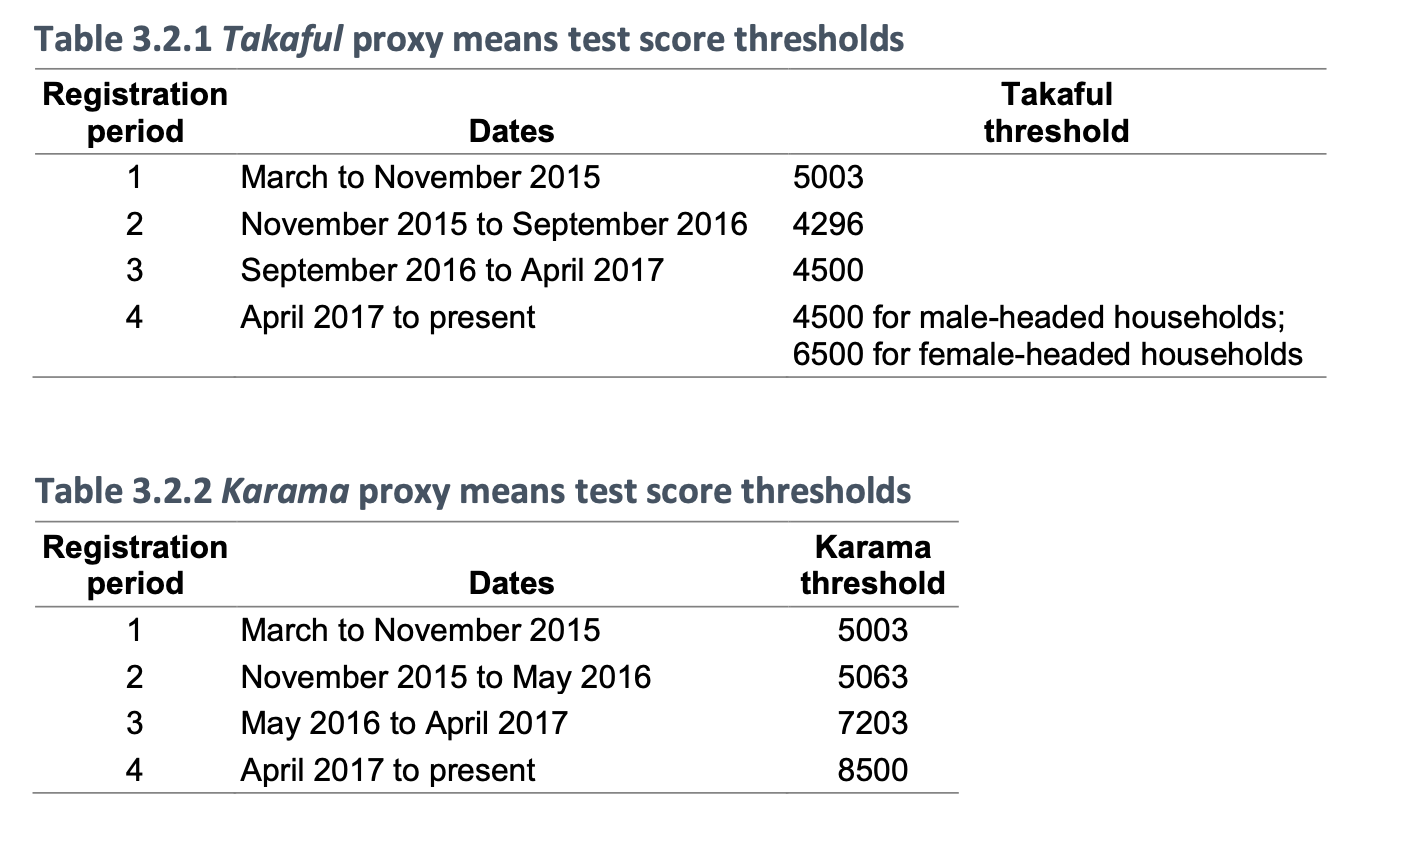
\includegraphics[width=0.8\textwidth]{./lecture_includes/takaful_table1.png}
        \caption{PMT thresholds over time for both programs}
    \end{figure}
\end{frame}

\begin{frame}{Fuzzy participation}

\begin{itemize}
\item Does not work, though, if administrators sometimes break the rules (i.e., it isn't followed perfectly)
\item Authors note that sometimes people who are eligible still won't participate (sometimes called ``non-compliance'')
\item Authors augment their study to account for this type of \emph{voluntary compliance} using ``fuzzy RDD'' 
\item But pretty sharp as you'll see, at least for one of the cutoffs (4.5)
\end{itemize}

\end{frame}

\subsection{Authors' findings}

\begin{frame}{Program Participation at 4.5 PMT}
    \begin{figure}
        \centering
        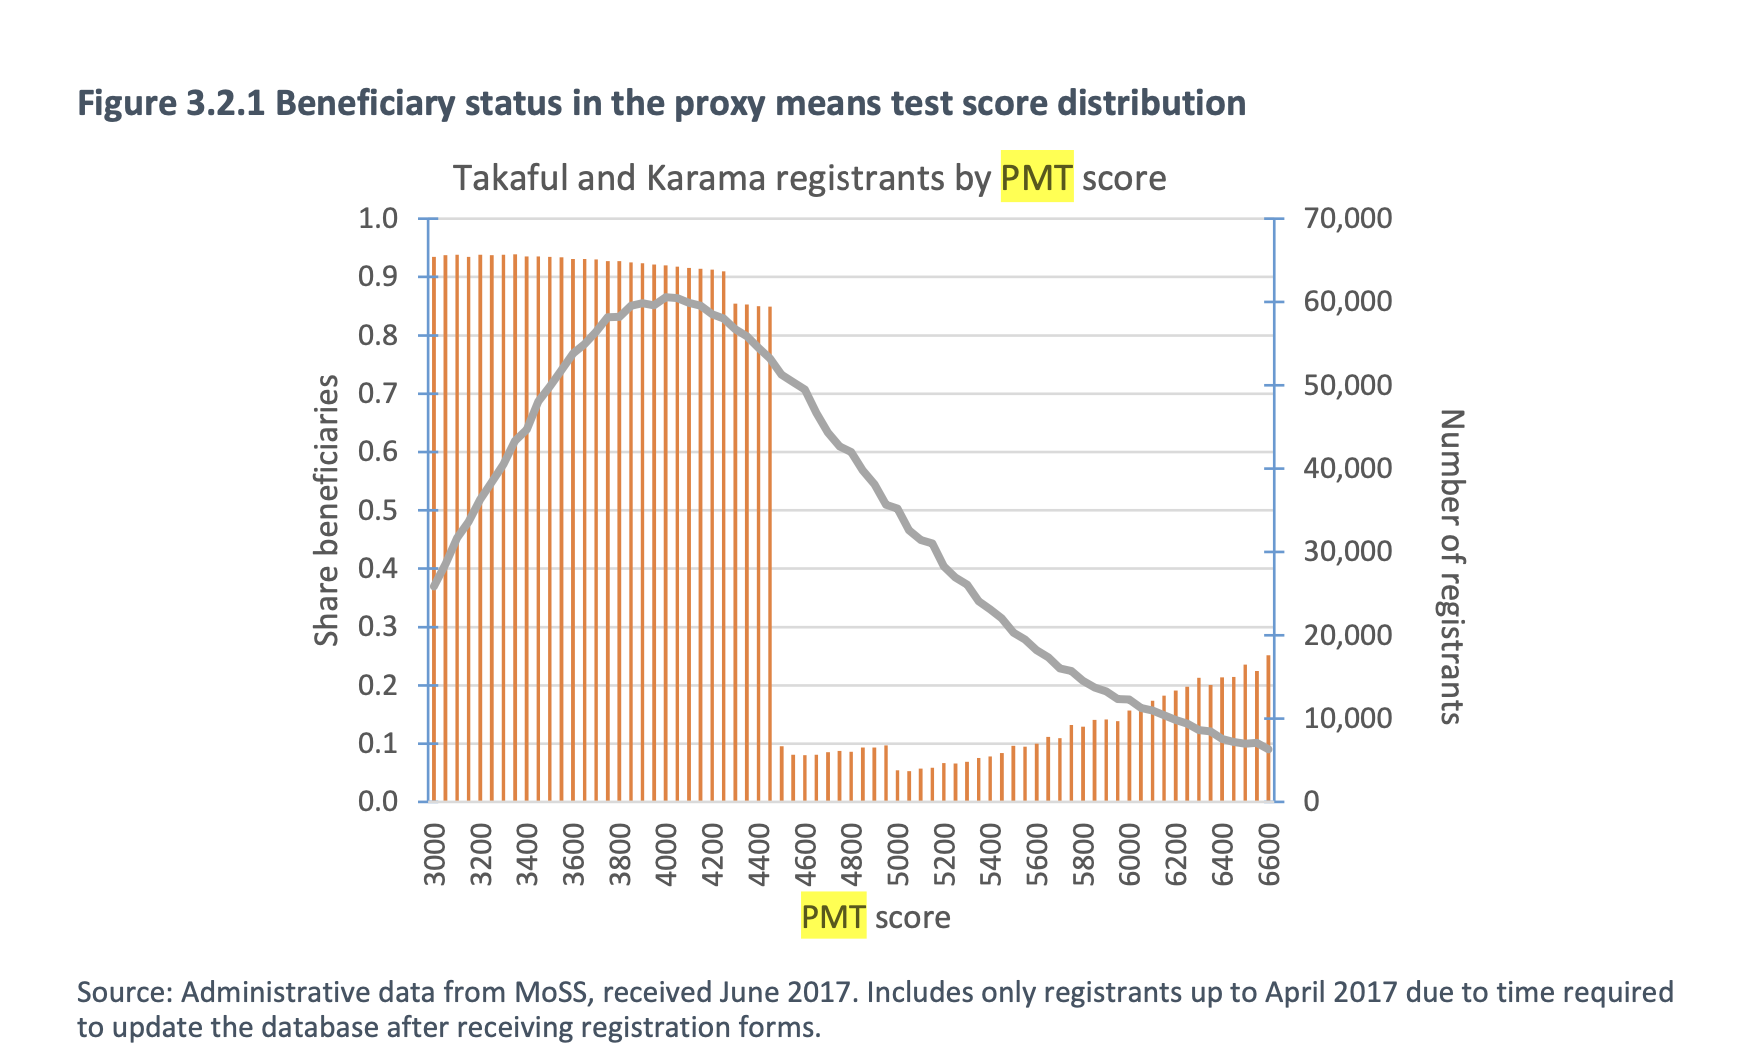
\includegraphics[width=0.8\textwidth]{./lecture_includes/takaful_density.png}
        \caption{Participation by score}
    \end{figure}
\end{frame}

\begin{frame}{Poverty (top), food and total spending (bottom)}
    \begin{figure}
        \centering
        \begin{minipage}{0.5\textwidth}
            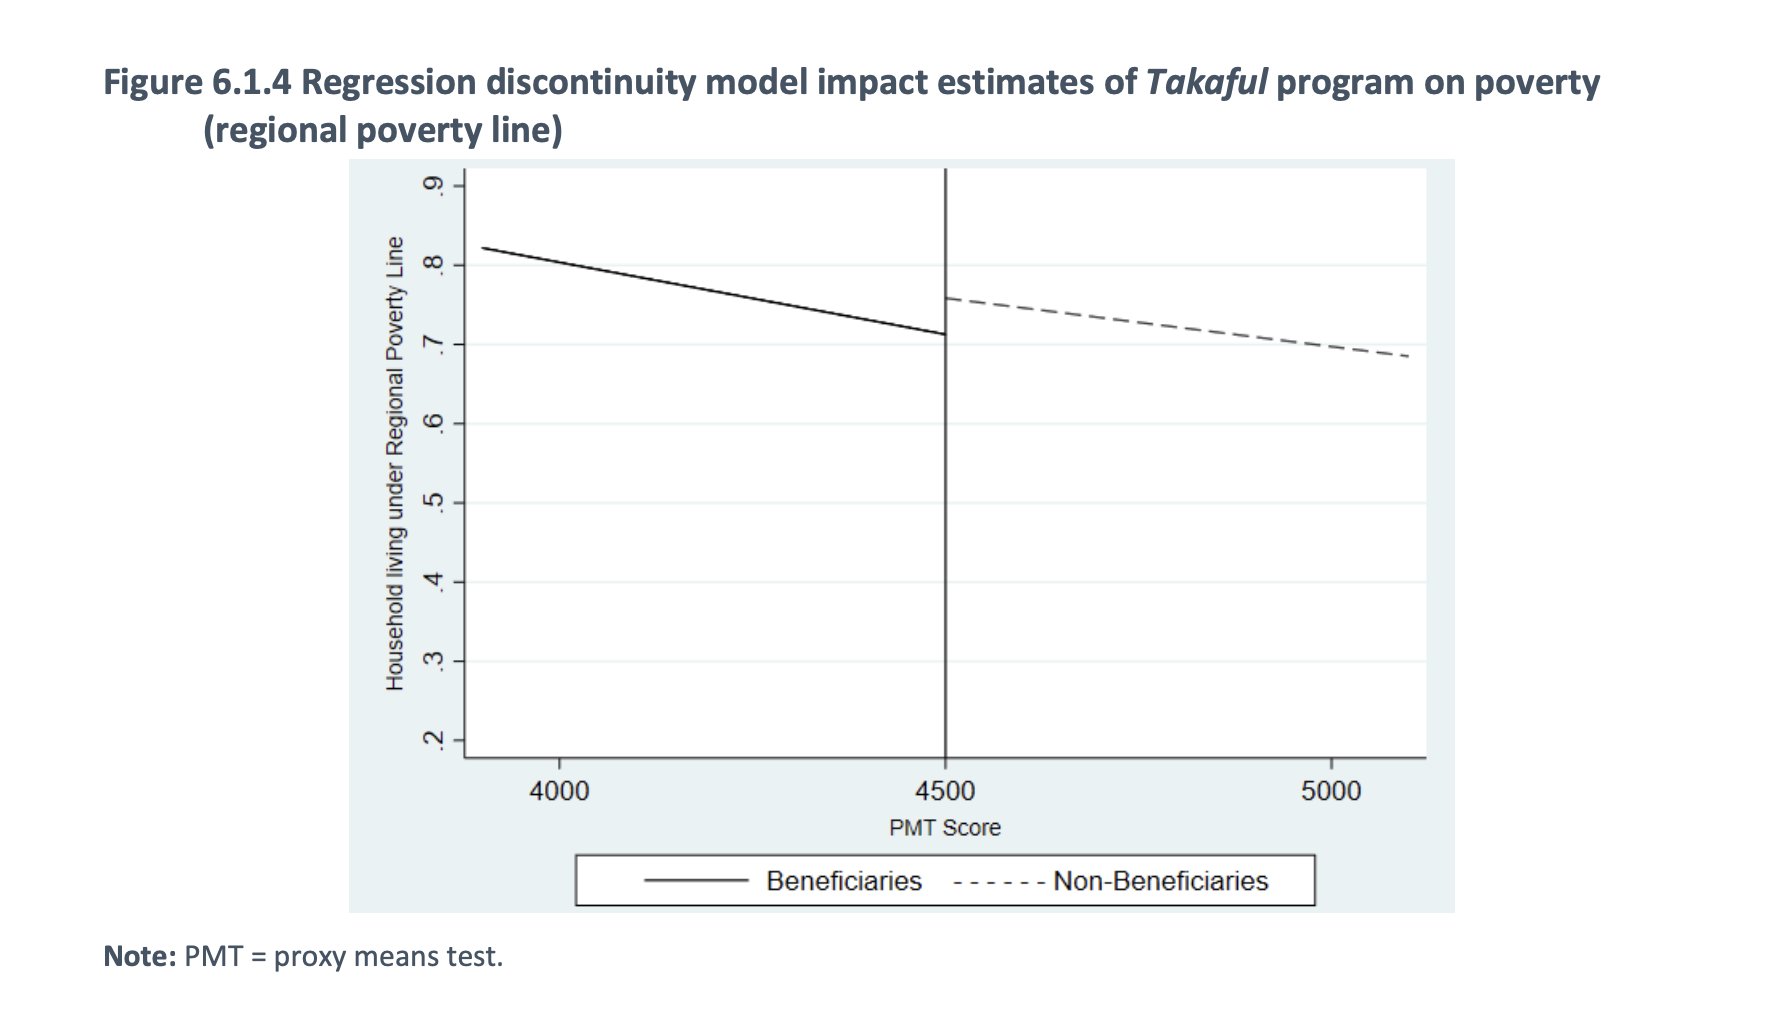
\includegraphics[width=\textwidth]{./lecture_includes/takaful_rdd4.png}
        \end{minipage}\hfill
        \begin{minipage}{0.5\textwidth}
            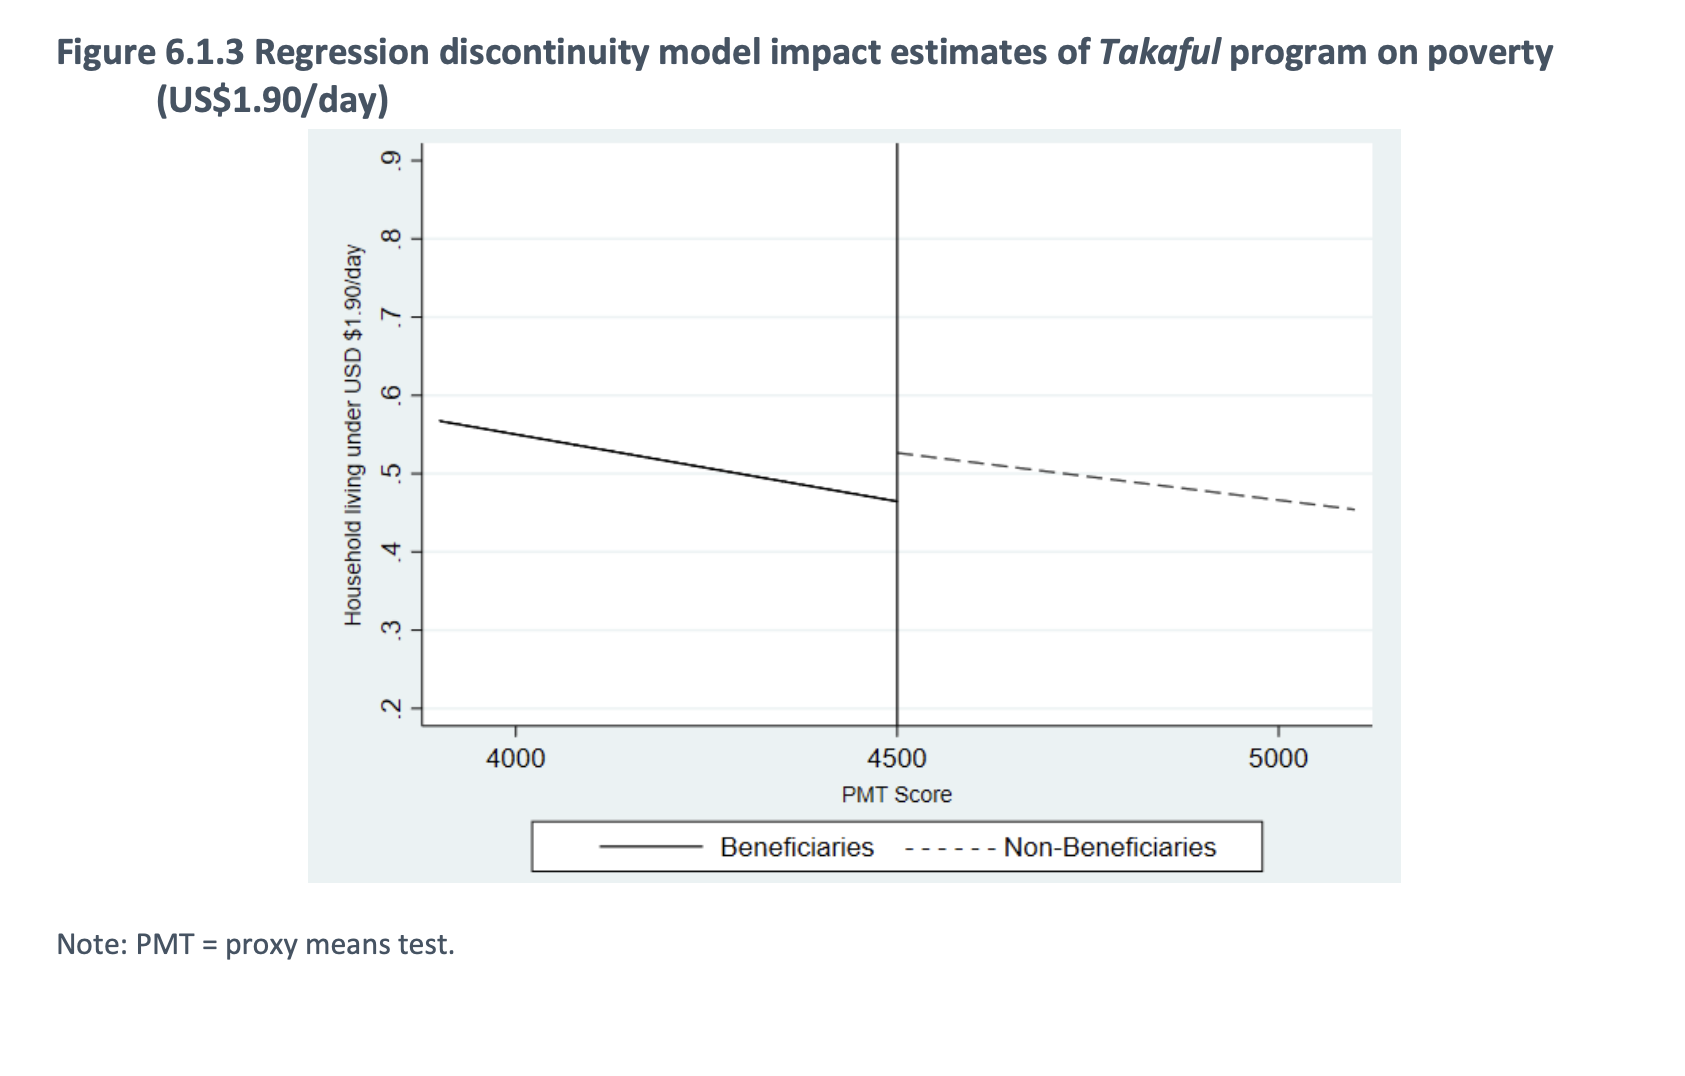
\includegraphics[width=\textwidth]{./lecture_includes/takaful_rdd3.png}
        \end{minipage}

        \vspace{0.5cm} % Adjust the vertical spacing if needed

        \begin{minipage}{0.5\textwidth}
            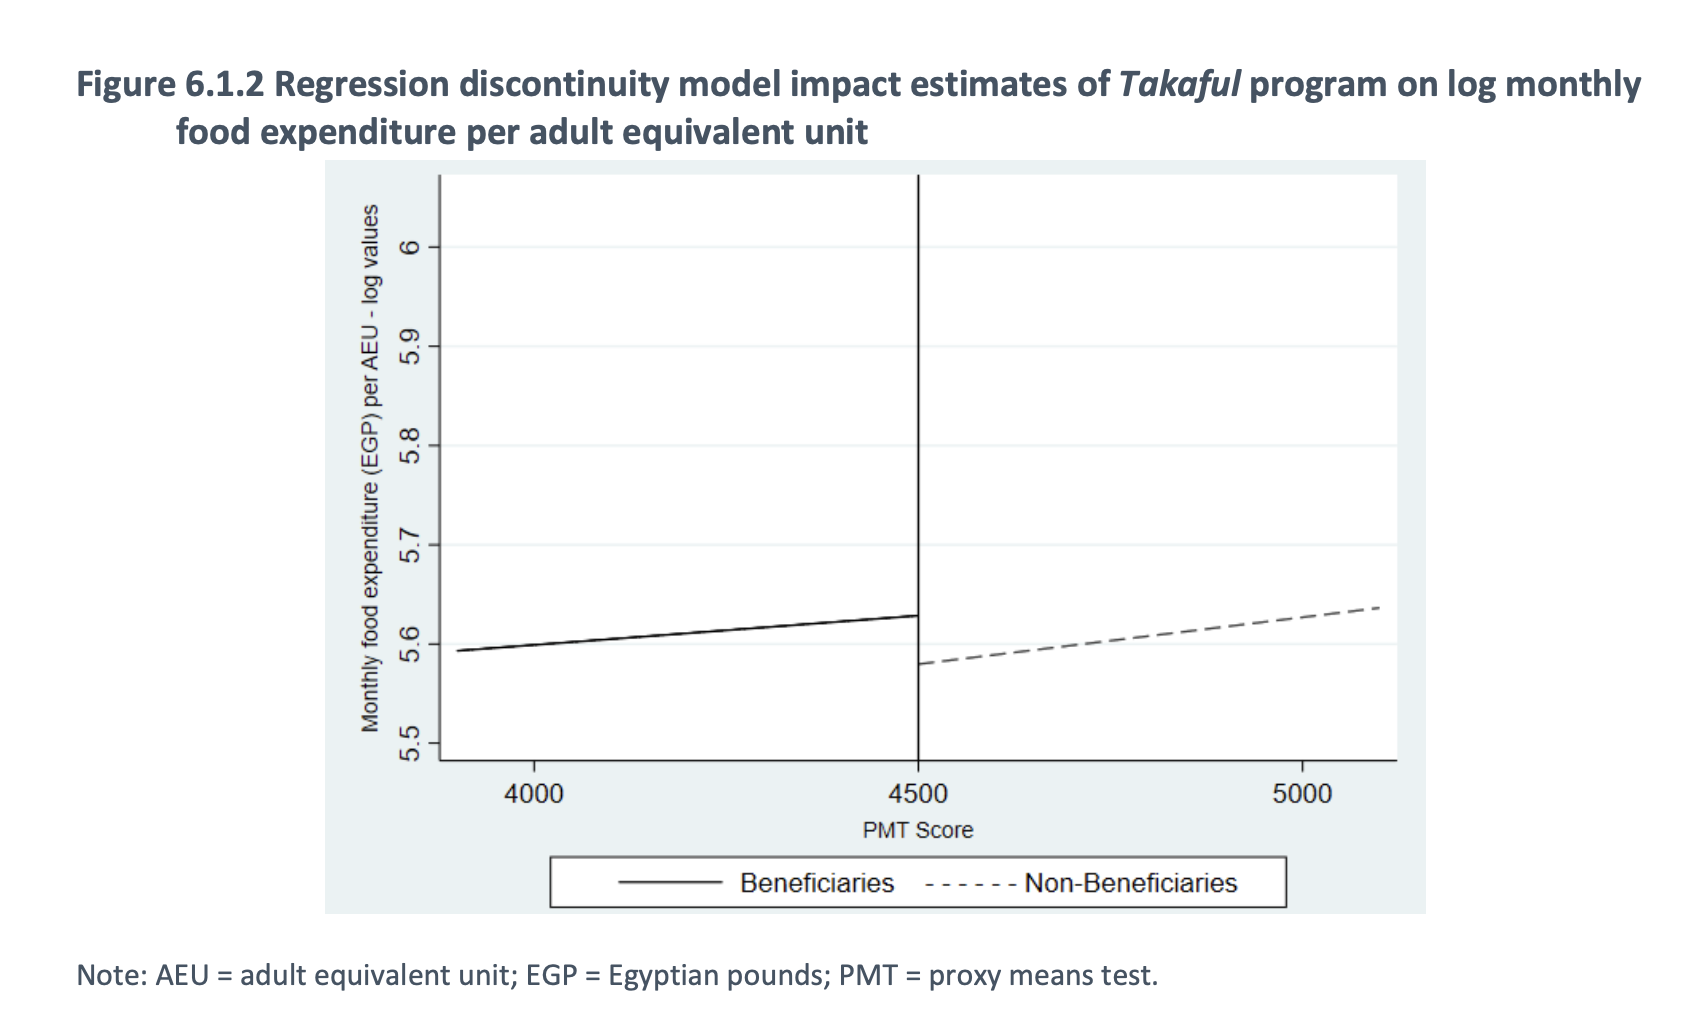
\includegraphics[width=\textwidth]{./lecture_includes/takaful_rdd2.png}
        \end{minipage}\hfill
        \begin{minipage}{0.5\textwidth}
            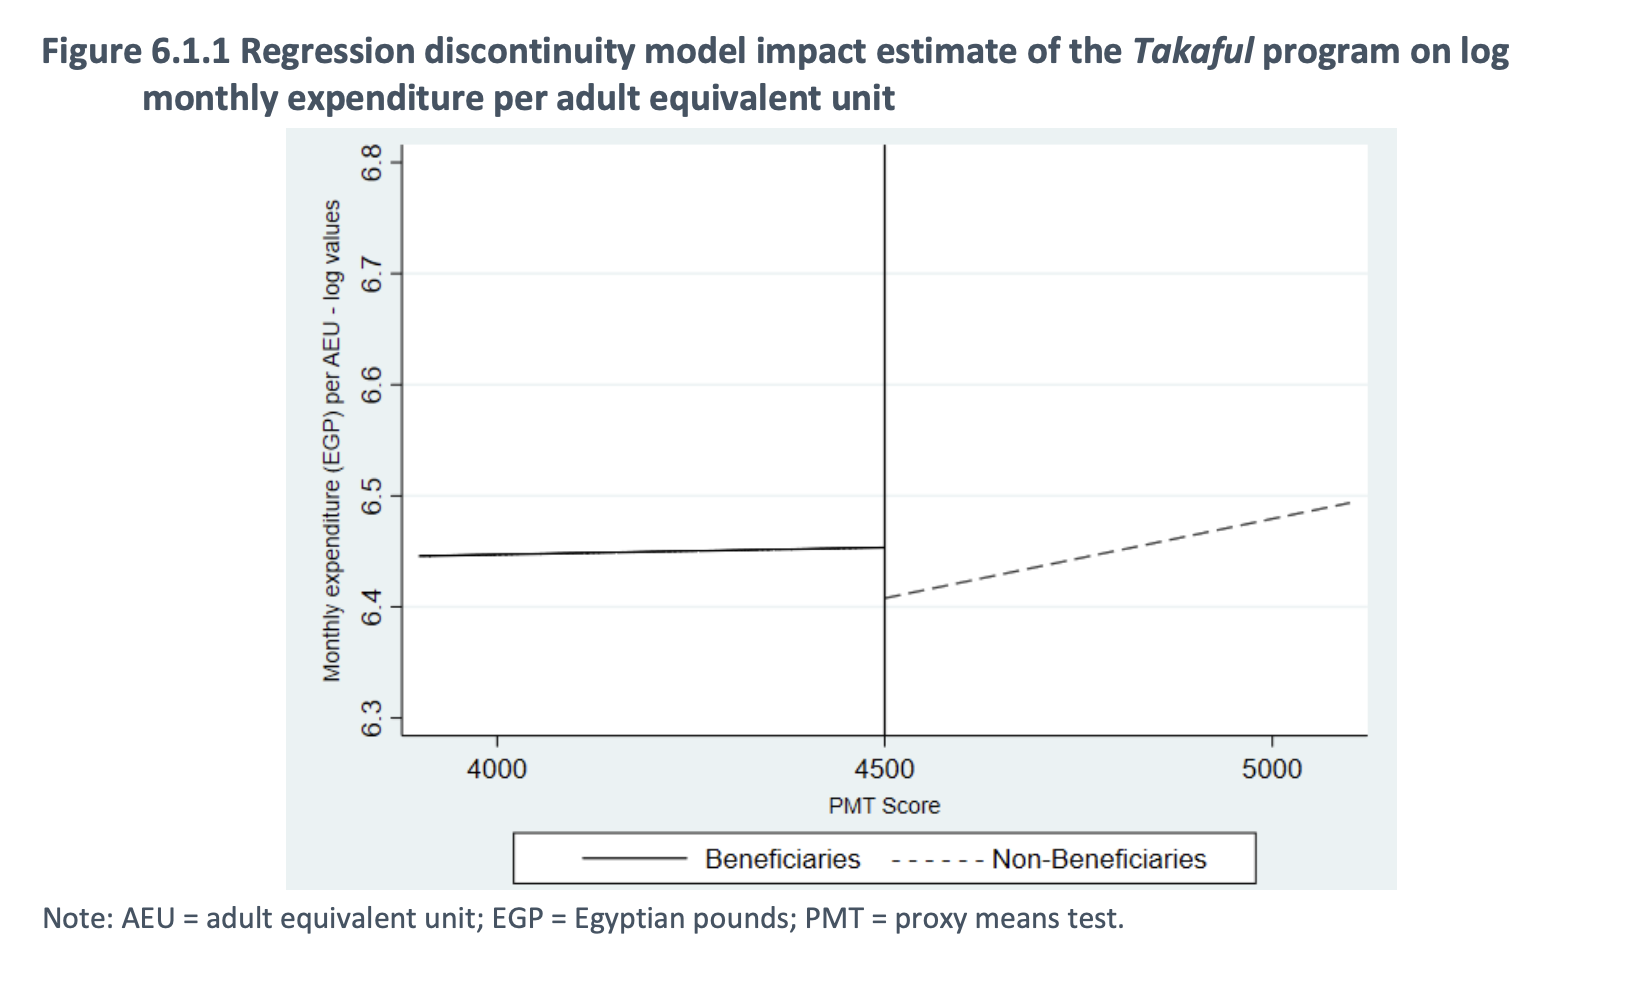
\includegraphics[width=\textwidth]{./lecture_includes/takaful_rdd1.png}
        \end{minipage}
    \end{figure}
\end{frame}


\begin{frame}{Summary}

\begin{itemize}
\item Some effects are clearer than others

	\begin{itemize}
	\item Large effects on food spending (around 8\%) and total spending (around 9\%)
	\item Large reductions in poverty (around 12\% reduction in living under poverty line)
	\item Huge effects on child ``weight-for-length/height'' (30-40\% SD) and reduced malnourishment (3-4\%)
	\end{itemize}
\item Some effects, particularly on food and clothes spending are unclear
	\begin{itemize}
	\item Increased consumption of fruit (around 25\%) but this is a little noisy and only shows up for one model
	\item Large increases in meat consumption (around 30-40\%)
	\item Some evidence for increased spending on clothes but also noisy
	\end{itemize}
\item Inconsistent evidence for optimism about future, spending on schooling, but some paradoxes like weakened female bargaining power over children schooling and healthcare
\end{itemize}

\end{frame}




\subsection{Comments and suggestions}

\begin{frame}{Comments}

\begin{itemize}
\item Very thorough, very contemporary, very interesting, very valuable -- highly encourage people to study it carefully, and re-evaluations done to confirm, as many good news (but lots of null results too)
\item RDD with and without fuzzy design paint a picture that around 4.5 there are some improvements from Takaful participation
\item But some things are strange too -- like worsened female bargaining power around child welfare, which I think makes this a somewhat intriguing finding meriting more research later
\item Much stronger evidence for Takaful than Karama, which is also puzzling

\end{itemize}

\end{frame}

\begin{frame}{Local impact is for some; average impact for everyone}

\begin{itemize}
\item Authors estimate a ``local'' average causal effect of the program \emph{at the thresholds only} and this is a strength and limitation
\item We can only learn impact for people who just barely missed and barely got in at 4.5, as opposed to all program participants, and policy choices should be based on everyone
\item If there is large differences in program effects, then this will not be informative about program's average effect (external validity), and policy should be judged by everyone, not just a thin slice at some arbitrary cutoff
%\item Means the finding has \emph{internal validity} (i.e., they found an average effect) but it lacks \emph{external validity} unless everyone has that same effect
\item Future work will need to try evaluate effects on everyone to determine to what degree that is the case which will require moving away from RDD 
\end{itemize}

\end{frame}


\begin{frame}{More pictures needed}

\begin{itemize}
\item To really communicate the findings, I think the authors need to find a way to communicate these results without so many tables
\item They may want to consider presenting the results using a boxplot of coefficients after normalizing scores into $z$-scores everywhere (see the following example)
\item This could help summarize the results as 150 pages is being chewed up by tons and tons of tables
\item RDD plots are hard to evaluate without scatter plot means along the bandwidth -- is this noise? Is this linear like they show?

\end{itemize}

\end{frame}

\begin{frame}{Example of $z$-score box plots from another paper}
    \begin{figure}
        \centering
        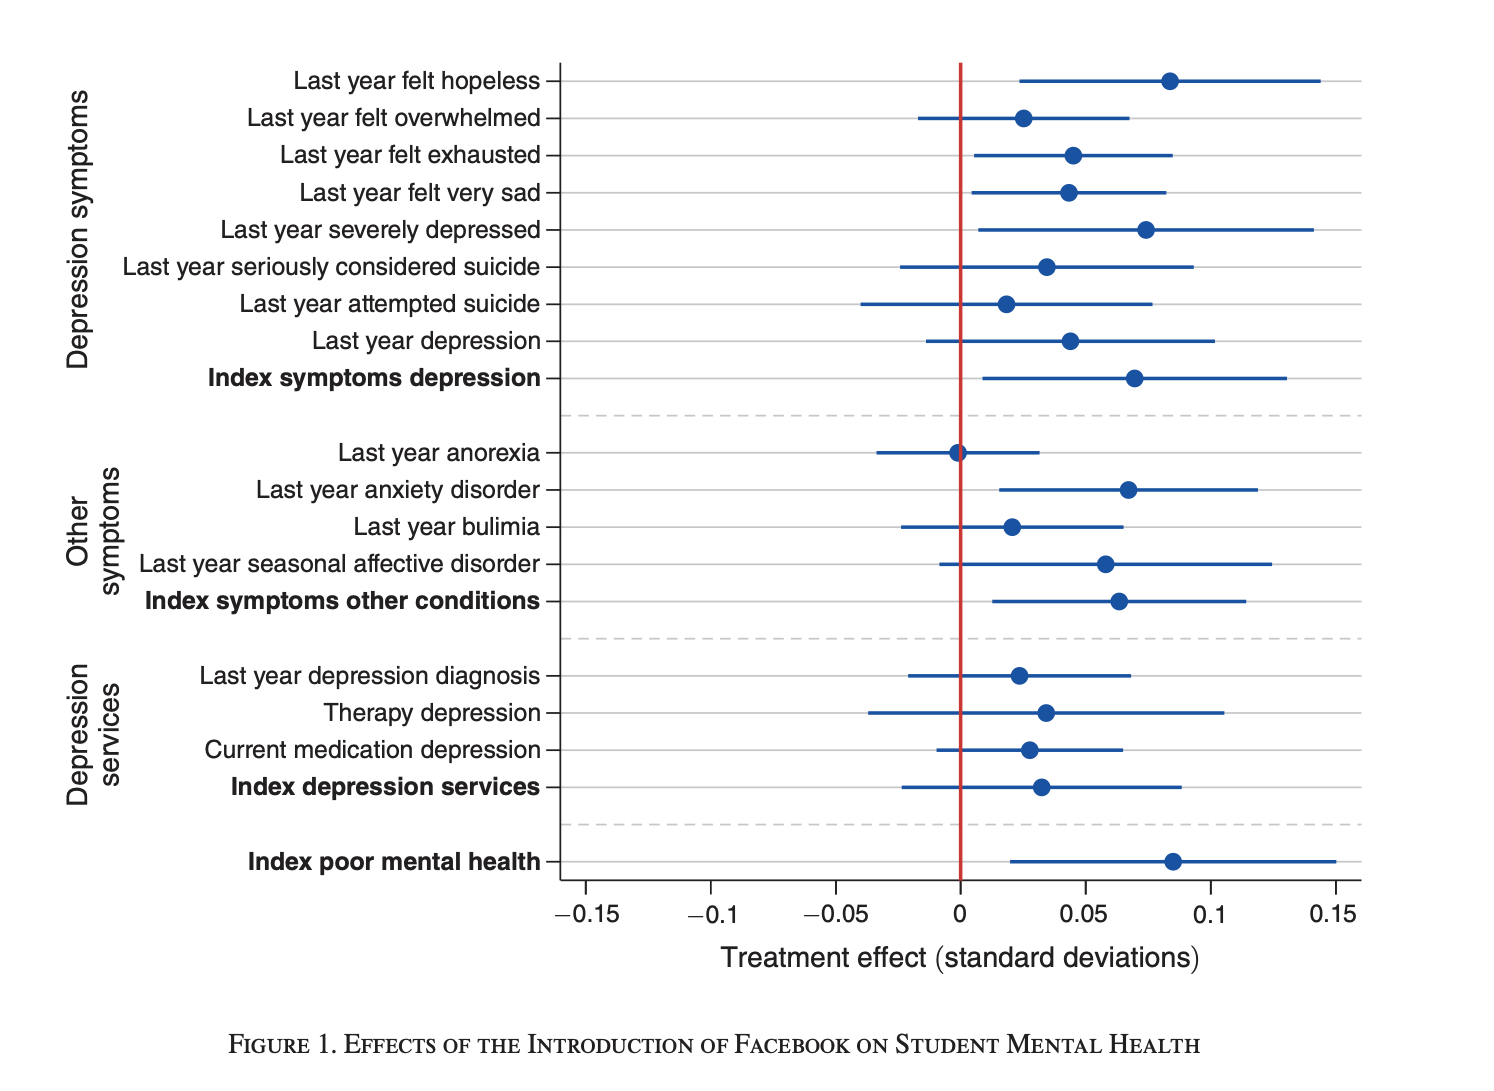
\includegraphics[width=0.8\textwidth]{./lecture_includes/facebook_2.png}
        \caption{Example of alternative data visualization}
    \end{figure}
\end{frame}


\begin{frame}{Comments on fuzzy model}

\begin{itemize}
\item Strongest instrument seems to be the 4.5 threshold, but authors are using multiple thresholds
\item Would prefer to see a single eligibility threshold with a re-centered running PMT score so they can interact eligibility with score, as this is just identified which makes first stage tests easier and weakness less a problem
\item Doing so will give a \emph{single instrument} which will minimize biases due to weak instruments (unclear strength of first stage beyond 4.5 PMT)
\item Another reason is it is inappropriate to use either the conventional or heteroskedasticity robust F-test for evaluating first stage strength 
\end{itemize}

\end{frame}

\begin{frame}{Comments on fuzzy model}

\begin{itemize}
\item First and second stage of instrumental variables should have same controls, but authors only control for strata in second stage according to their equation
\item Highly encourage the authors to use IV models like \texttt{ivregress 2sls} in Stata (or equivalent in R) so that this is guaranteed
\item Consider controlling for score and a quadratic in score to model nonlinearities because ultimately RDD ``extrapolates'' based on the functional form and they may have underfitting
\end{itemize}

\end{frame}


\begin{frame}{Strengths and implications}

\begin{itemize}
\item Paper's strengths are its rigor and focus on strong methods for overcoming selection bias
\item Some findings stronger than others
\item Policymakers can consider studying programs using these methods, and should, but keep in mind limitations and challenges in inference
\item Causal inference methodologies have advanced in the non-randomized setting, but have not replaced the controlled randomization and never will
\end{itemize}

\end{frame}

\begin{frame}{Credible Causal Inference and Parting Remarks}

\begin{itemize}

\item Validity in causal inference is based on methods that reflect the reality of why people entered a program (i.e., all methods are equally scientific)
\item Fuzzy RDD \emph{only} estimates the "local average treatment effect" which is only the average effect for people at 4.5 (internal but not external validity unless effects are the same for everyone)
\item Future avenues need to examine the average effect for \emph{all participants} as treatment effect heterogeneity could strengthen or weaken results found at 4.5
participants
\item Machine learning methods, such as causal forests and double debiased machine learning, can do this, but require a lot of information on observable confounders related to participation and outcomes
\item \textcolor{blue}{Thank you!!}

\end{itemize}

\end{frame}

% Mention that the first stage regression equation needs to interact the threshold with the score and examine both the linear and second order polynomials
% Mention too that the second stage will need to have the same  controls as the first, and it doesn't appear that it does.  Authors seem to not control for the score in the second stage.  IV models use the same covariate controls in both stages,  Highly encourage the authors to use -ivregress 2sls- in Stata or equivalent in R. 



\end{document}



I have just one final comment. At the conclusion of the presentation, it would be highly beneficial to outline the next steps or the way forward. This should involve mentioning specific advanced methods or techniques that have the potential to yield better results and address the limitations of IFPRI's assessment. Such an addition could open doors to future projects. In our experience, all participants will be eager to hear about the possibility of conducting scenario analysis (what-if) to measure the potential impact of different program designs or policy alternatives.


% ---- Content ----

% 20 min. no more than 20 slides (15 ideally). The goal is to keep the audience's attention 

% 7 min of causal inference as a methodology
% advances in this line of work --> more specific impact assessment
% 10 min commenting on the study, the type of assessment that took place
% "based on what I've seen, Causal Infernce in its newest version, it can give more room for answering questions about impact of programs".  Position causal inference within the impact evaluation methodology.  It can do "1 2 3 4 5" and then show examples.  First 10 minutes.  

% goal: to formulate a program (expensive currently to Egyptian government).  We need to know the proper assessment.  Are the methodologies proper enough to justify how much money is being spent? 
% my advantage is that I am an outsider; I'm watching it but talking about it from my own expertise.
% Other panelists will speak about the study they undertook.  We want to know what they are doing -- everyone is involved in the assessment (JPAL, for instance).  Some of the panelists will be critical (e.g., an anthropologist may be critical).  I can use examples.  But use examples to illustrate the methodologies using benign topics that aren't offensive or polarizing.  
% What can be done with quasi-experimental methodologies versus what I have seen being assessed.  I want to open doors.  They're going to put in a proposal for an assessment of the program. 

% Can I discuss "treatment assignment mechanism" but without so much detail?  And can I drop the potential outcomes material and just assume the average treatment effect. 

% Be critical of the study, say what I think what kinds of improvements can be done.  

% I won't need to explain the program as that'll be described before my talk.  Go into an assessment of its impact. Cost benefit is important for normative questions.

% Use as a thread the program so that I wrap people into this idea.  

% Common errors for conclusions for not understanding.  I need entry points for grabbing people. 